\documentclass[border=4pt]{standalone}
% Preámbulo común de las figuras. Cada figura es un documento standalone
% que se compila a SVG con scripts/build_figures.sh
\usepackage[utf8]{inputenc}
\usepackage{amsmath}
\usepackage{tikz}
\usepackage[american, siunitx]{circuitikz}
\usetikzlibrary{arrows.meta,calc,decorations.pathmorphing,patterns}
\tikzset{
  >={Stealth[length=2.2mm]},
  eje/.style={->, thin},
  hilo/.style={thick},
}
% Paleta común: tonos medios legibles sobre fondo claro
\definecolor{azul}{RGB}{31,94,168}
\definecolor{rojo}{RGB}{192,57,43}
\definecolor{verde}{RGB}{39,128,73}
\definecolor{naranja}{RGB}{211,120,30}
\definecolor{morado}{RGB}{125,60,152}

\begin{document}
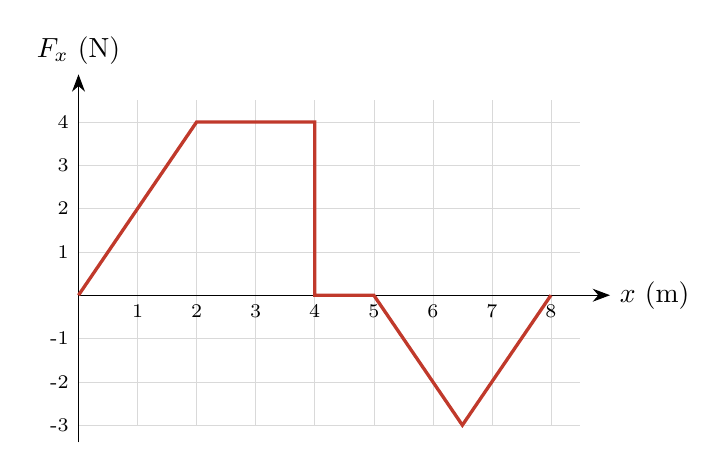
\begin{tikzpicture}[xscale=0.75, yscale=0.55]
  \draw[step=1, gray!30, very thin] (0,-3) grid (8.5,4.5);
  \draw[eje] (0,0) -- (9,0) node[right]{$x$ (m)};
  \draw[eje] (0,-3.4) -- (0,5.1) node[above]{$F_x$ (N)};
  \foreach \x in {1,...,8} \node[below, font=\scriptsize] at (\x,0) {\x};
  \foreach \y in {-3,-2,-1,1,2,3,4} \node[left, font=\scriptsize] at (0,\y) {\y};
  \draw[very thick, rojo] (0,0) -- (2,4) -- (4,4) -- (4,0) -- (5,0) -- (6.5,-3) -- (8,0);
\end{tikzpicture}
\end{document}
